\documentclass{article}

\usepackage[cmex10]{amsmath}
\usepackage{subcaption}

\usepackage{tikz}

\definecolor{alizarin}{RGB}{231, 76, 60}
\definecolor{pomegranate}{RGB}{192, 57, 43}
\definecolor{emerald}{RGB}{46, 204, 113}
\definecolor{turquoise}{RGB}{26, 188, 156}
\definecolor{greensea}{RGB}{22, 160, 133}

\begin{document}

\begin{figure}[h]
    \centering
    \captionsetup{justification=centering}
    \begin{subfigure}{0.3\textwidth}
        \centering
        \resizebox{\textwidth}{!}{%
        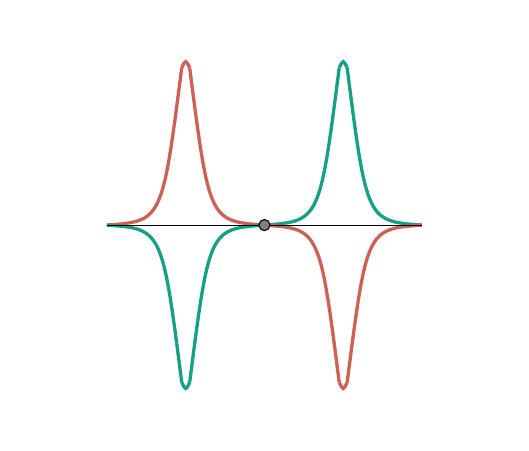
\begin{tikzpicture}
            % ON Center
            \draw[color=pomegranate!80, very thick] (-2.00, 0.00) .. controls (-1.30, 0.05) .. (-1.05, 2.00);
            \draw[color=pomegranate!80, very thick] (-1.05, 2.00) .. controls (-1.00, 2.10) .. (-0.95, 2.00);
            \draw[color=pomegranate!80, very thick] ( 0.00, 0.00) .. controls (-0.70, 0.05) .. (-0.95, 2.00);
            % OFF Surround
            \draw[color=greensea,       very thick] (-2.00, 0.00) .. controls (-1.30,-0.05) .. (-1.05,-2.00);
            \draw[color=greensea,       very thick] (-1.05,-2.00) .. controls (-1.00,-2.10) .. (-0.95,-2.00);
            \draw[color=greensea,       very thick] ( 0.00, 0.00) .. controls (-0.70,-0.05) .. (-0.95,-2.00);
            % ON Center
            \draw[color=greensea,       very thick] ( 0.00, 0.00) .. controls ( 0.70, 0.05) .. ( 0.95, 2.00);
            \draw[color=greensea,       very thick] ( 1.05, 2.00) .. controls ( 1.00, 2.10) .. ( 0.95, 2.00);
            \draw[color=greensea,       very thick] ( 2.00, 0.00) .. controls ( 1.30, 0.05) .. ( 1.05, 2.00);
            % OFF Surround
            \draw[color=pomegranate!80, very thick] ( 0.00, 0.00) .. controls ( 0.70,-0.05) .. ( 0.95,-2.00);
            \draw[color=pomegranate!80, very thick] ( 1.05,-2.00) .. controls ( 1.00,-2.10) .. ( 0.95,-2.00);
            \draw[color=pomegranate!80, very thick] ( 2.00, 0.00) .. controls ( 1.30,-0.05) .. ( 1.05,-2.00);
            % Reference line & point
            \draw (-2,0) -- (2,0);
            \filldraw[color=black, fill=gray] ( 0.00, 0.00) circle (2pt);
            % Frame to ensure alignment
            \draw[color=white] (-3.0, 2.5) rectangle (3.0, -2.5);
        \end{tikzpicture}}
    \end{subfigure}
    \begin{subfigure}{0.3\textwidth}
        \resizebox{\textwidth}{!}{%
        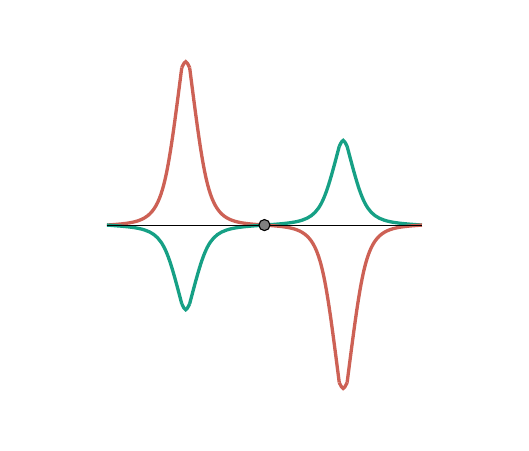
\begin{tikzpicture}
            % ON Center
            \draw[color=pomegranate!80, very thick] (-2.00, 0.00) .. controls (-1.30, 0.05) .. (-1.05, 2.00);
            \draw[color=pomegranate!80, very thick] (-1.05, 2.00) .. controls (-1.00, 2.10) .. (-0.95, 2.00);
            \draw[color=pomegranate!80, very thick] ( 0.00, 0.00) .. controls (-0.70, 0.05) .. (-0.95, 2.00);
            % OFF Surround
            \draw[color=greensea,       very thick] (-2.00, 0.00) .. controls (-1.30,-0.05) .. (-1.05,-1.00);
            \draw[color=greensea,       very thick] (-1.05,-1.00) .. controls (-1.00,-1.10) .. (-0.95,-1.00);
            \draw[color=greensea,       very thick] ( 0.00, 0.00) .. controls (-0.70,-0.05) .. (-0.95,-1.00);
            % ON Center
            \draw[color=greensea,       very thick] ( 0.00, 0.00) .. controls ( 0.70, 0.05) .. ( 0.95, 1.00);
            \draw[color=greensea,       very thick] ( 1.05, 1.00) .. controls ( 1.00, 1.10) .. ( 0.95, 1.00);
            \draw[color=greensea,       very thick] ( 2.00, 0.00) .. controls ( 1.30, 0.05) .. ( 1.05, 1.00);
            % OFF Surround
            \draw[color=pomegranate!80, very thick] ( 0.00, 0.00) .. controls ( 0.70,-0.05) .. ( 0.95,-2.00);
            \draw[color=pomegranate!80, very thick] ( 1.05,-2.00) .. controls ( 1.00,-2.10) .. ( 0.95,-2.00);
            \draw[color=pomegranate!80, very thick] ( 2.00, 0.00) .. controls ( 1.30,-0.05) .. ( 1.05,-2.00);
            % Reference line & point
            \draw (-2,0) -- (2,0);
            \filldraw[color=black, fill=gray] ( 0.00, 0.00) circle (2pt);
            % Frame to ensure alignment
            \draw[color=white] (-3.0, 2.5) rectangle (3.0, -2.5);
        \end{tikzpicture}}
    \end{subfigure}
    \begin{subfigure}{0.3\textwidth}
        \resizebox{\textwidth}{!}{%
        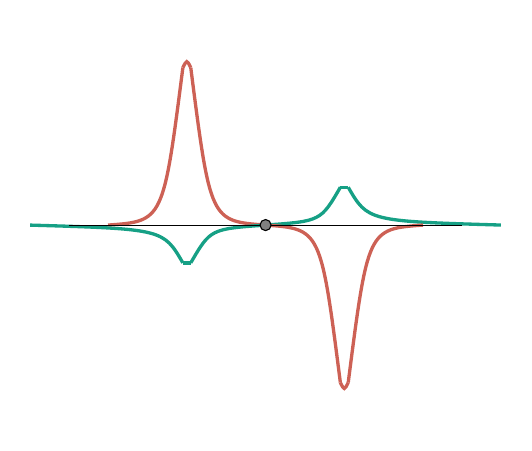
\begin{tikzpicture}
            % ON Center
            \draw[color=pomegranate!80, very thick] (-2.00, 0.00) .. controls (-1.30, 0.05) .. (-1.05, 2.00);
            \draw[color=pomegranate!80, very thick] (-1.05, 2.00) .. controls (-1.00, 2.10) .. (-0.95, 2.00);
            \draw[color=pomegranate!80, very thick] ( 0.00, 0.00) .. controls (-0.70, 0.05) .. (-0.95, 2.00);
            % OFF Surround
            \draw[color=greensea,       very thick] (-3.00, 0.00) .. controls (-1.30,-0.05) .. (-1.05,-0.48);
            \draw[color=greensea,       very thick] (-1.05,-0.48) .. controls (-1.00,-0.49) .. (-0.95,-0.48);
            \draw[color=greensea,       very thick] ( 0.00, 0.00) .. controls (-0.70,-0.05) .. (-0.95,-0.48);
            % ON Center
            \draw[color=greensea,       very thick] ( 0.00, 0.00) .. controls ( 0.70, 0.05) .. ( 0.95, 0.48);
            \draw[color=greensea,       very thick] ( 1.05, 0.48) .. controls ( 1.00, 0.49) .. ( 0.95, 0.48);
            \draw[color=greensea,       very thick] ( 3.00, 0.00) .. controls ( 1.30, 0.05) .. ( 1.05, 0.48);
            % OFF Surround
            \draw[color=pomegranate!80, very thick] ( 0.00, 0.00) .. controls ( 0.70,-0.05) .. ( 0.95,-2.00);
            \draw[color=pomegranate!80, very thick] ( 1.05,-2.00) .. controls ( 1.00,-2.10) .. ( 0.95,-2.00);
            \draw[color=pomegranate!80, very thick] ( 2.00, 0.00) .. controls ( 1.30,-0.05) .. ( 1.05,-2.00);
            % Reference line & point
            \draw (-2.5,0) -- (2.5,0);
            \filldraw[color=black, fill=gray] ( 0.00, 0.00) circle (2pt);
            % Frame to ensure alignment
            \draw[color=white] (-3.0, 2.5) rectangle (3.0, -2.5);
        \end{tikzpicture}}
    \end{subfigure}
\end{figure}
        
% FIGURE: Single-opponent recpetive field cross section
\begin{figure}[h]
    \centering
    \captionsetup{justification=centering}
    \begin{subfigure}{0.3\textwidth}
        \centering
        \resizebox{\textwidth}{!}{%
        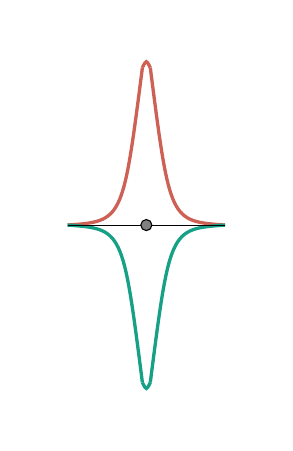
\begin{tikzpicture}
            % ON Center
            \draw[color=pomegranate!80, very thick] (-1.00, 0.00) .. controls (-0.30, 0.05) .. (-0.05, 2.00);
            \draw[color=pomegranate!80, very thick] (-0.05, 2.00) .. controls ( 0.00, 2.10) .. ( 0.05, 2.00);
            \draw[color=pomegranate!80, very thick] ( 1.00, 0.00) .. controls ( 0.30, 0.05) .. ( 0.05, 2.00);
            % OFF Surround
            \draw[color=greensea, very thick] (-1.00, 0.00) .. controls (-0.30,-0.05) .. (-0.05,-2.00);
            \draw[color=greensea, very thick] (-0.05,-2.00) .. controls ( 0.00,-2.10) .. ( 0.05,-2.00);
            \draw[color=greensea, very thick] ( 1.00, 0.00) .. controls ( 0.30,-0.05) .. ( 0.05,-2.00);
            % Reference line & point
            \draw (-1,0) -- (1,0);
            \filldraw[color=black, fill=gray] ( 0.00, 0.00) circle (2pt);
            % Frame to ensure alignment
            \draw[color=white] (-1.5, 2.5) rectangle (1.5, -2.5);
        \end{tikzpicture}}
        \caption{Symmetric balanced \\ single opponent \\ receptive field}
    \end{subfigure}%
    \begin{subfigure}{0.3\textwidth}
        \centering
        \resizebox{\textwidth}{!}{%
        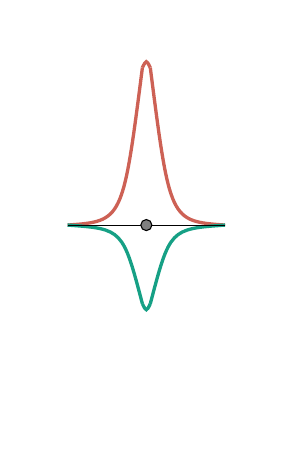
\begin{tikzpicture}
            % ON Center
            \draw[color=pomegranate!80, very thick] (-1.00, 0.00) .. controls (-0.30, 0.05) .. (-0.05, 2.00);
            \draw[color=pomegranate!80, very thick] (-0.05, 2.00) .. controls ( 0.00, 2.10) .. ( 0.05, 2.00);
            \draw[color=pomegranate!80, very thick] ( 1.00, 0.00) .. controls ( 0.30, 0.05) .. ( 0.05, 2.00);
            % OFF Surround
            \draw[color=greensea,       very thick] (-1.00, 0.00) .. controls (-0.30,-0.05) .. (-0.05,-1.00);
            \draw[color=greensea,       very thick] (-0.05,-1.00) .. controls ( 0.00,-1.10) .. ( 0.05,-1.00);
            \draw[color=greensea,       very thick] ( 1.00, 0.00) .. controls ( 0.30,-0.05) .. ( 0.05,-1.00);
            % Reference line & point
            \draw (-1,0) -- (1,0);
            \filldraw[color=black, fill=gray] ( 0.00, 0.00) circle (2pt);
            % Frame to ensure alignment
            \draw[color=white] (-1.5, 2.5) rectangle (1.5, -2.5);
        \end{tikzpicture}}
        \caption{Symmetric imbalanced \\ single opponent \\ receptive field}
    \end{subfigure}%
    \begin{subfigure}{0.3\textwidth}
        \centering
        \resizebox{\textwidth}{!}{%
        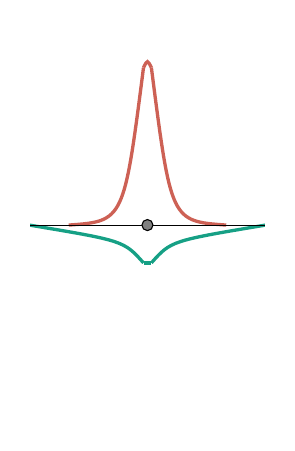
\begin{tikzpicture}
            % ON Center
            \draw[color=pomegranate!80, very thick] (-1.00, 0.00) .. controls (-0.30, 0.05) .. (-0.05, 2.00);
            \draw[color=pomegranate!80, very thick] (-0.05, 2.00) .. controls ( 0.00, 2.10) .. ( 0.05, 2.00);
            \draw[color=pomegranate!80, very thick] ( 1.00, 0.00) .. controls ( 0.30, 0.05) .. ( 0.05, 2.00);
            % OFF Surround
            \draw[color=greensea,       very thick] (-1.50, 0.00) .. controls (-0.30,-0.20) .. (-0.05,-0.48);
            \draw[color=greensea,       very thick] (-0.05,-0.48) .. controls ( 0.00,-0.49) .. ( 0.05,-0.48);
            \draw[color=greensea,       very thick] ( 1.50, 0.00) .. controls ( 0.30,-0.20) .. ( 0.05,-0.48);
            % Reference line & point
            \draw (-1.5,0) -- (1.5,0);
            \filldraw[color=black, fill=gray]       ( 0.00, 0.00) circle (2pt);
            % Frame to ensure alignment
            \draw[color=white]                      (-1.5, 2.5) rectangle (1.5, -2.5);
        \end{tikzpicture}}
        \caption{Center/surround \\ single opponent \\ receptive field}
    \end{subfigure}%
\end{figure}


% FIGURE: Oriented double-opponent receptive fields
\begin{figure}[h] \label{fig:dos}
    \centering
    \captionsetup{justification=centering}
    % Horizontal Double-Opponent Receptive Fields
    \begin{subfigure}{0.5\textwidth}
        \centering
        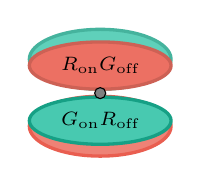
\begin{tikzpicture}
            \filldraw[color=greensea!80,    fill=turquoise!70, very thick]( 0.00, 1.43) ellipse   (0.90 and 0.38);
            \filldraw[color=alizarin!90,    fill=alizarin!70,  very thick]( 0.00, 0.58) ellipse   (0.90 and 0.38);
            \filldraw[color=pomegranate!80, fill=alizarin!80,  very thick]( 0.00, 1.35) ellipse   (0.90 and 0.30)
                 node[color=black, anchor=center] {$\scriptstyle R_{\text{on}}G_{\text{off}}$};
            \filldraw[color=greensea,       fill=turquoise!80, very thick]( 0.00, 0.65) ellipse   (0.90 and 0.30)
                 node[color=black, anchor=center] {$\scriptstyle G_{\text{on}}R_{\text{off}}$};
            \filldraw[color=black,          fill=gray]                    ( 0.00, 1.00) circle    (2pt);
        \end{tikzpicture}
        \caption{Vertical $R$ vs. $G$ double-opponent \\ cell receptive fields.}
    \end{subfigure}%
    \begin{subfigure}{0.5\textwidth}
        \centering
        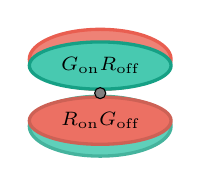
\begin{tikzpicture}
            \filldraw[color=alizarin!90,    fill=alizarin!70,  very thick]( 0.00, 1.43) ellipse   (0.90 and 0.38);
            \filldraw[color=greensea!80,    fill=turquoise!70, very thick]( 0.00, 0.58) ellipse   (0.90 and 0.38);
            \filldraw[color=greensea,       fill=turquoise!80, very thick]( 0.00, 1.35) ellipse   (0.90 and 0.30)
                 node[color=black, anchor=center] {$\scriptstyle G_{\text{on}}R_{\text{off}}$};
            \filldraw[color=pomegranate!80, fill=alizarin!80,  very thick]( 0.00, 0.65) ellipse   (0.90 and 0.30)
                 node[color=black, anchor=center] {$\scriptstyle R_{\text{on}}G_{\text{off}}$};
            \filldraw[color=black,          fill=gray]                    ( 0.00, 1.00) circle    (2pt);
        \end{tikzpicture}
        \caption{Vertical $G$ vs. $R$ double-opponent \\ cell receptive fields.}
    \end{subfigure}%
    \par \bigskip
    % Diagonal Double-Opponent Receptive Fields #1
    \begin{subfigure}{0.5\textwidth}
        \centering
        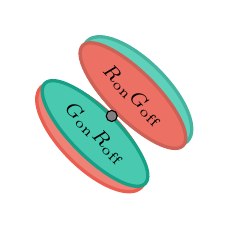
\begin{tikzpicture}
            \filldraw[color=greensea!80,    fill=turquoise!70, very thick, rotate=45]( 1.16, 0.70) ellipse   (0.38 and 0.90);
            \filldraw[color=alizarin!90,    fill=alizarin!70,  very thick, rotate=45]( 0.33, 0.70) ellipse   (0.38 and 0.90);
            \filldraw[color=pomegranate!80, fill=alizarin!80,  very thick, rotate=45]( 1.08, 0.70) ellipse   (0.30 and 0.90)
                 node[color=black, anchor=center, rotate=-45] {$\scriptstyle R_{\text{on}}G_{\text{off}}$};
            \filldraw[color=greensea,       fill=turquoise!80, very thick, rotate=45]( 0.40, 0.70) ellipse   (0.30 and 0.90)
                 node[color=black, anchor=center, rotate=-45] {$\scriptstyle G_{\text{on}}R_{\text{off}}$};
            \filldraw[color=black,          fill=gray]                    ( 0.00, 1.00) circle    (2pt);
        \end{tikzpicture}
        \caption{Diagonal $R$ vs. $G$ double-opponent \\ cell receptive fields.}
    \end{subfigure}%
    \begin{subfigure}{0.5\textwidth}
        \centering
        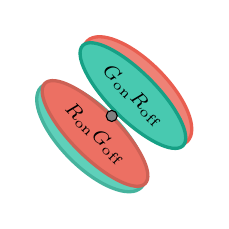
\begin{tikzpicture}
            \filldraw[color=alizarin!90,    fill=alizarin!70,  very thick, rotate=45]( 1.16, 0.70) ellipse   (0.38 and 0.90);
            \filldraw[color=greensea!80,    fill=turquoise!70, very thick, rotate=45]( 0.33, 0.70) ellipse   (0.38 and 0.90);
            \filldraw[color=greensea,       fill=turquoise!80, very thick, rotate=45]( 1.08, 0.70) ellipse   (0.30 and 0.90)
                 node[color=black, anchor=center, rotate=-45] {$\scriptstyle G_{\text{on}}R_{\text{off}}$};
            \filldraw[color=pomegranate!80, fill=alizarin!80,  very thick, rotate=45]( 0.40, 0.70) ellipse   (0.30 and 0.90)
                 node[color=black, anchor=center, rotate=-45] {$\scriptstyle R_{\text{on}}G_{\text{off}}$};
            \filldraw[color=black,          fill=gray]                    ( 0.00, 1.00) circle    (2pt);
        \end{tikzpicture}
        \caption{Diagonal $G$ vs. $R$ double-opponent \\ cell receptive fields.}
    \end{subfigure}%
    \par \bigskip
    % Vertical Double-Opponent Receptive Fields
    \begin{subfigure}{0.5\textwidth}
        \centering
        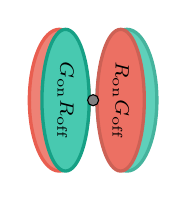
\begin{tikzpicture}
            \filldraw[color=greensea!80,    fill=turquoise!70, very thick]( 0.43, 1.00) ellipse   (0.38 and 0.90);
            \filldraw[color=alizarin!90,    fill=alizarin!70,  very thick](-0.43, 1.00) ellipse   (0.38 and 0.90);
            \filldraw[color=pomegranate!80, fill=alizarin!80,  very thick]( 0.35, 1.00) ellipse   (0.30 and 0.90)
                 node[color=black, anchor=center, rotate=-90] {$\scriptstyle R_{\text{on}}G_{\text{off}}$};
            \filldraw[color=greensea,       fill=turquoise!80, very thick](-0.35, 1.00) ellipse   (0.30 and 0.90)
                 node[color=black, anchor=center, rotate=-90] {$\scriptstyle G_{\text{on}}R_{\text{off}}$};
            \filldraw[color=black,          fill=gray]                    ( 0.00, 1.00) circle    (2pt);
        \end{tikzpicture}
        \caption{Horizontal $R$ vs. $G$ double-opponent \\ cell receptive fields.}
    \end{subfigure}%
    \begin{subfigure}{0.5\textwidth}
        \centering
        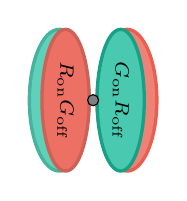
\begin{tikzpicture}
            \filldraw[color=alizarin!90,    fill=alizarin!70,  very thick]( 0.43, 1.00) ellipse   (0.38 and 0.90);
            \filldraw[color=greensea!80,    fill=turquoise!70, very thick](-0.43, 1.00) ellipse   (0.38 and 0.90);
            \filldraw[color=greensea,       fill=turquoise!80, very thick]( 0.35, 1.00) ellipse   (0.30 and 0.90)
                 node[color=black, anchor=center, rotate=-90] {$\scriptstyle G_{\text{on}}R_{\text{off}}$};
            \filldraw[color=pomegranate!80, fill=alizarin!80,  very thick](-0.35, 1.00) ellipse   (0.30 and 0.90)
                 node[color=black, anchor=center, rotate=-90] {$\scriptstyle R_{\text{on}}G_{\text{off}}$};
            \filldraw[color=black,          fill=gray]                    ( 0.00, 1.00) circle    (2pt);
        \end{tikzpicture}
        \caption{Horizontal $G$ vs. $R$ double-opponent \\ cell receptive fields.}
    \end{subfigure}%
    \par \bigskip
    % Diagonal Double-Opponent Receptive Fields #2
    \begin{subfigure}{0.5\textwidth}
        \centering
        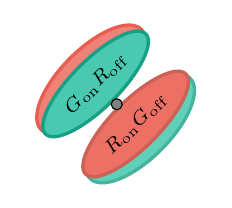
\begin{tikzpicture}
            \filldraw[color=alizarin!90,    fill=alizarin!70, very thick, rotate=45]( 0.70, 1.16) ellipse   (0.90 and 0.38);
            \filldraw[color=greensea!80,    fill=turquoise!70,  very thick, rotate=45]( 0.70, 0.28) ellipse   (0.90 and 0.38);
            \filldraw[color=greensea,       fill=turquoise!80,  very thick, rotate=45]( 0.70, 1.08) ellipse   (0.90 and 0.30)
                 node[color=black, anchor=center, rotate=45] {$\scriptstyle G_{\text{on}}R_{\text{off}}$};
            \filldraw[color=pomegranate!80, fill=alizarin!80, very thick, rotate=45]( 0.70, 0.36) ellipse   (0.90 and 0.30)
                 node[color=black, anchor=center, rotate=45] {$\scriptstyle R_{\text{on}}G_{\text{off}}$};
            \filldraw[color=black,          fill=gray]                    ( 0.00, 1.00) circle    (2pt);
        \end{tikzpicture}
        \caption{Diagonal $R$ vs. $G$ double-opponent \\ cell receptive fields.}
    \end{subfigure}%
    \begin{subfigure}{0.5\textwidth}
        \centering
        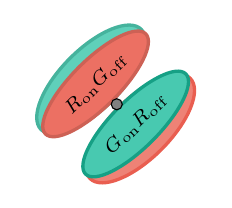
\begin{tikzpicture}
            \filldraw[color=greensea!80,    fill=turquoise!70, very thick, rotate=45]( 0.70, 1.16) ellipse   (0.90 and 0.38);
            \filldraw[color=alizarin!90,    fill=alizarin!70,  very thick, rotate=45]( 0.70, 0.28) ellipse   (0.90 and 0.38);
            \filldraw[color=pomegranate!80, fill=alizarin!80,  very thick, rotate=45]( 0.70, 1.08) ellipse   (0.90 and 0.30)
                 node[color=black, anchor=center, rotate=45] {$\scriptstyle R_{\text{on}}G_{\text{off}}$};
            \filldraw[color=greensea,       fill=turquoise!80, very thick, rotate=45]( 0.70, 0.36) ellipse   (0.90 and 0.30)
                 node[color=black, anchor=center, rotate=45] {$\scriptstyle G_{\text{on}}R_{\text{off}}$};
            \filldraw[color=black,          fill=gray]                    ( 0.00, 1.00) circle    (2pt);
        \end{tikzpicture}
        \caption{Diagonal $R$ vs. $G$ double-opponent \\ cell receptive fields.}
    \end{subfigure}%
    \caption{sean is cool}
\end{figure}


% FIGURE: horizontal red/green double-opponent cell on horizontal red/green border
\begin{figure}[h] \label{fig:do-orient-h}
    \begin{subfigure}{0.3\textwidth}
        \centering
        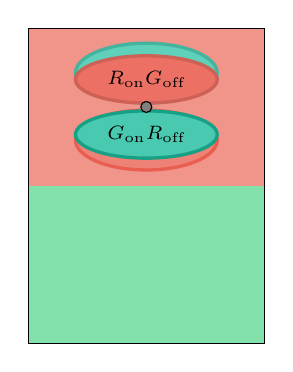
\begin{tikzpicture}
            \fill[alizarin!60]                                            (-1.50, 2.00) rectangle (1.50, 0.00);
            \fill[emerald!60]                                             (-1.50,-2.00) rectangle (1.50, 0.00);
            \filldraw[color=greensea!80,    fill=turquoise!70, very thick]( 0.00, 1.43) ellipse   (0.90 and 0.38);
            \filldraw[color=alizarin!90,    fill=alizarin!70,  very thick]( 0.00, 0.58) ellipse   (0.90 and 0.38);
            \filldraw[color=pomegranate!80, fill=alizarin!80,  very thick]( 0.00, 1.35) ellipse   (0.90 and 0.30)
                 node[color=black, anchor=center] {$\scriptstyle R_{\text{on}}G_{\text{off}}$};
            \filldraw[color=greensea,       fill=turquoise!80, very thick]( 0.00, 0.65) ellipse   (0.90 and 0.30)
                 node[color=black, anchor=center] {$\scriptstyle G_{\text{on}}R_{\text{off}}$};
            \filldraw[color=black,          fill=gray]                    ( 0.00, 1.00) circle    (2pt);
            \draw (current bounding box.north east) rectangle (current bounding box.south west);
        \end{tikzpicture}
        \caption{Minor Response}
    \end{subfigure}%
    \begin{subfigure}{0.3\textwidth}
        \centering
        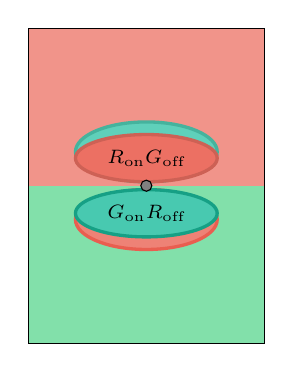
\begin{tikzpicture}
            \fill[alizarin!60]                                            (-1.50, 2.00) rectangle (1.50, 0.00);
            \fill[emerald!60]                                             (-1.50,-2.00) rectangle (1.50, 0.00);
            \filldraw[color=greensea!80,    fill=turquoise!70, very thick]( 0.00, 0.43) ellipse   (0.90 and 0.38);
            \filldraw[color=alizarin!90,    fill=alizarin!70,  very thick]( 0.00,-0.43) ellipse   (0.90 and 0.38);
            \filldraw[color=pomegranate!80, fill=alizarin!80,  very thick]( 0.00, 0.35) ellipse   (0.90 and 0.30)
                 node[color=black, anchor=center] {$\scriptstyle R_{\text{on}}G_{\text{off}}$};
            \filldraw[color=greensea,       fill=turquoise!80, very thick]( 0.00,-0.35) ellipse   (0.90 and 0.30)
                 node[color=black, anchor=center] {$\scriptstyle G_{\text{on}}R_{\text{off}}$};
            \filldraw[color=black,          fill=gray]                    ( 0.00, 0.00) circle    (2pt);
        \draw (current bounding box.north east) rectangle (current bounding box.south west);
        \end{tikzpicture}
        \caption{Maximum Response}
    \end{subfigure}%
    \begin{subfigure}{0.3\textwidth}
        \centering
        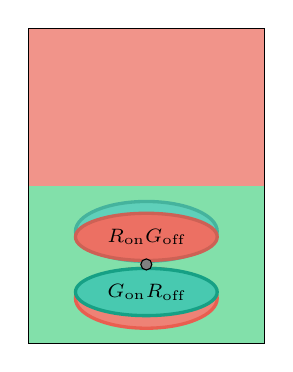
\begin{tikzpicture}
            \fill[alizarin!60]                                            (-1.50, 2.00) rectangle (1.50, 0.00);
            \fill[emerald!60]                                             (-1.50,-2.00) rectangle (1.50, 0.00);
            \filldraw[color=greensea!80,    fill=turquoise!70, very thick]( 0.00,-0.58) ellipse   (0.90 and 0.38);
            \filldraw[color=alizarin!90,    fill=alizarin!70,  very thick]( 0.00,-1.43) ellipse   (0.90 and 0.38);
            \filldraw[color=pomegranate!80, fill=alizarin!80,  very thick]( 0.00,-0.65) ellipse   (0.90 and 0.30)
                 node[color=black, anchor=center] {$\scriptstyle R_{\text{on}}G_{\text{off}}$};
            \filldraw[color=greensea,       fill=turquoise!80, very thick]( 0.00,-1.35) ellipse   (0.90 and 0.30)
                 node[color=black, anchor=center] {$\scriptstyle G_{\text{on}}R_{\text{off}}$};
            \filldraw[color=black,          fill=gray]                    ( 0.00,-1.00) circle    (2pt);
        \draw (current bounding box.north east) rectangle (current bounding box.south west);
        \end{tikzpicture}
        \caption{Minor Response}
    \end{subfigure}%
    \par \bigskip
    \begin{subfigure}{0.3\textwidth}
        \centering
        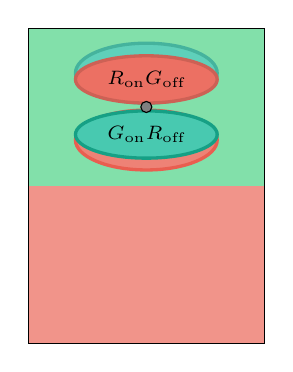
\begin{tikzpicture}
            \fill[emerald!60]                                             (-1.50, 2.00) rectangle (1.50, 0.00);
            \fill[alizarin!60]                                            (-1.50,-2.00) rectangle (1.50, 0.00);
            \filldraw[color=greensea!80,    fill=turquoise!70, very thick]( 0.00, 1.43) ellipse   (0.90 and 0.38);
            \filldraw[color=alizarin!90,    fill=alizarin!70,  very thick]( 0.00, 0.58) ellipse   (0.90 and 0.38);
            \filldraw[color=pomegranate!80, fill=alizarin!80,  very thick]( 0.00, 1.35) ellipse   (0.90 and 0.30)
                 node[color=black, anchor=center] {$\scriptstyle R_{\text{on}}G_{\text{off}}$};
            \filldraw[color=greensea,       fill=turquoise!80, very thick]( 0.00, 0.65) ellipse   (0.90 and 0.30)
                 node[color=black, anchor=center] {$\scriptstyle G_{\text{on}}R_{\text{off}}$};
            \filldraw[color=black,          fill=gray]                    ( 0.00, 1.00) circle    (2pt);
            \draw (current bounding box.north east) rectangle (current bounding box.south west);
        \end{tikzpicture}
        \caption{Minor Response}
    \end{subfigure}%
    \begin{subfigure}{0.3\textwidth}
        \centering
        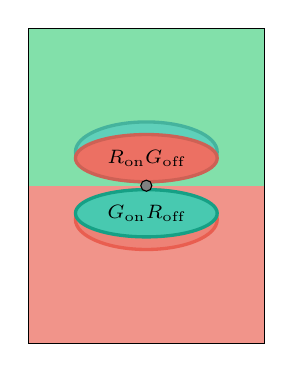
\begin{tikzpicture}
            \fill[emerald!60]                                             (-1.50, 2.00) rectangle (1.50, 0.00);
            \fill[alizarin!60]                                            (-1.50,-2.00) rectangle (1.50, 0.00);
            \filldraw[color=greensea!80,    fill=turquoise!70, very thick]( 0.00, 0.43) ellipse   (0.90 and 0.38);
            \filldraw[color=alizarin!90,    fill=alizarin!70,  very thick]( 0.00,-0.43) ellipse   (0.90 and 0.38);
            \filldraw[color=pomegranate!80, fill=alizarin!80,  very thick]( 0.00, 0.35) ellipse   (0.90 and 0.30)
                 node[color=black, anchor=center] {$\scriptstyle R_{\text{on}}G_{\text{off}}$};
            \filldraw[color=greensea,       fill=turquoise!80, very thick]( 0.00,-0.35) ellipse   (0.90 and 0.30)
                 node[color=black, anchor=center] {$\scriptstyle G_{\text{on}}R_{\text{off}}$};
            \filldraw[color=black,          fill=gray]                    ( 0.00, 0.00) circle    (2pt);
        \draw (current bounding box.north east) rectangle (current bounding box.south west);
        \end{tikzpicture}
        \caption{No Response}
    \end{subfigure}%
    \begin{subfigure}{0.3\textwidth}
        \centering
        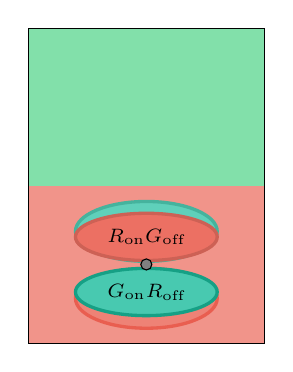
\begin{tikzpicture}
            \fill[emerald!60]                                             (-1.50, 2.00) rectangle (1.50, 0.00);
            \fill[alizarin!60]                                            (-1.50,-2.00) rectangle (1.50, 0.00);
            \filldraw[color=greensea!80,    fill=turquoise!70, very thick]( 0.00,-0.58) ellipse   (0.90 and 0.38);
            \filldraw[color=alizarin!90,    fill=alizarin!70,  very thick]( 0.00,-1.43) ellipse   (0.90 and 0.38);
            \filldraw[color=pomegranate!80, fill=alizarin!80,  very thick]( 0.00,-0.65) ellipse   (0.90 and 0.30)
                 node[color=black, anchor=center] {$\scriptstyle R_{\text{on}}G_{\text{off}}$};
            \filldraw[color=greensea,       fill=turquoise!80, very thick]( 0.00,-1.35) ellipse   (0.90 and 0.30)
                 node[color=black, anchor=center] {$\scriptstyle G_{\text{on}}R_{\text{off}}$};
            \filldraw[color=black,          fill=gray]                    ( 0.00,-1.00) circle    (2pt);
        \draw (current bounding box.north east) rectangle (current bounding box.south west);
        \end{tikzpicture}
        \caption{Minor Response}
    \end{subfigure}
    \caption{A double-opponent cell selective to horizontally oriented borders with red above and green below; only responsive to that particular stimulus. In Figure (b), the neuron is presented with its ideal stimulus: its $R_{\text{on}}$ and $G_{\text{on}}$ receptive fields are fully activated while its $R_{\text{off}}$ and $G_{\text{off}}$ receptive fields are completely unactivated. Figure (e) presents the neuron with the exact opposite stimulus, neither its $R_{\text{on}}$ nor $G_{\text{on}}$ receptive fields are activate at all, and both its $R_{\text{off}}$ and $G_{\text{off}}$ receptive fields are fully activated, ensuring no response possible from the cell. While its $R_{\text{on}}$ receptive field might be strongly stimulated in (a) and (f), it's $R_{\text{off}}$ receptive field cancels it out. Similarly, in (c) and (d) its $G_{\text{on}}$ receptive field is stimulated but cancelled out by activity in its $G_{\text{off}}$ receptive field.}
\end{figure}


% FIGURE: vertical red/green double-opponent cell on horizontal red/green border
\begin{figure}[h] \label{fig:do-orient-v}
    \begin{subfigure}{0.3\textwidth}
        \centering
        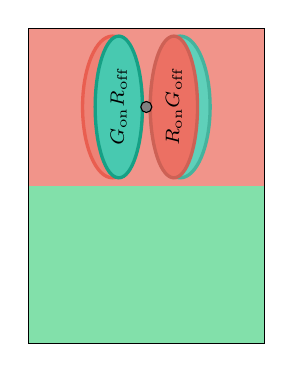
\begin{tikzpicture}
            \fill[alizarin!60]                                            (-1.50, 2.00) rectangle (1.50, 0.00);
            \fill[emerald!60]                                             (-1.50,-2.00) rectangle (1.50, 0.00);
            \filldraw[color=greensea!80,    fill=turquoise!70, very thick]( 0.43, 1.00) ellipse   (0.38 and 0.90);
            \filldraw[color=alizarin!90,    fill=alizarin!70,  very thick](-0.43, 1.00) ellipse   (0.38 and 0.90);
            \filldraw[color=pomegranate!80, fill=alizarin!80,  very thick]( 0.35, 1.00) ellipse   (0.30 and 0.90)
                 node[color=black, anchor=center, rotate=90] {$\scriptstyle R_{\text{on}}G_{\text{off}}$};
            \filldraw[color=greensea,       fill=turquoise!80, very thick](-0.35, 1.00) ellipse   (0.30 and 0.90)
                 node[color=black, anchor=center, rotate=90] {$\scriptstyle G_{\text{on}}R_{\text{off}}$};
            \filldraw[color=black,          fill=gray]                    ( 0.00, 1.00) circle    (2pt);
            \draw (current bounding box.north east) rectangle (current bounding box.south west);
        \end{tikzpicture}
        \caption{Minor Response}
    \end{subfigure}%
    \begin{subfigure}{0.3\textwidth}
        \centering
            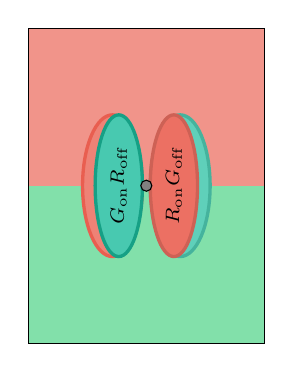
\begin{tikzpicture}
            \fill[alizarin!60]                                            (-1.50, 2.00) rectangle (1.50, 0.00);
            \fill[emerald!60]                                             (-1.50,-2.00) rectangle (1.50, 0.00);
            \filldraw[color=greensea!80,    fill=turquoise!70, very thick]( 0.43, 0.00) ellipse   (0.38 and 0.90);
            \filldraw[color=alizarin!90,    fill=alizarin!70,  very thick](-0.43, 0.00) ellipse   (0.38 and 0.90);
            \filldraw[color=pomegranate!80, fill=alizarin!80,  very thick]( 0.35, 0.00) ellipse   (0.30 and 0.90)
                 node[color=black, anchor=center, rotate=90] {$\scriptstyle R_{\text{on}}G_{\text{off}}$};
            \filldraw[color=greensea,       fill=turquoise!80, very thick](-0.35, 0.00) ellipse   (0.30 and 0.90)
                 node[color=black, anchor=center, rotate=90] {$\scriptstyle G_{\text{on}}R_{\text{off}}$};
            \filldraw[color=black,          fill=gray]                    ( 0.00, 0.00) circle    (2pt);
            \draw (current bounding box.north east) rectangle (current bounding box.south west);
            \end{tikzpicture}
        \caption{Minimal Response}
    \end{subfigure}%
    \begin{subfigure}{0.3\textwidth}
        \centering
            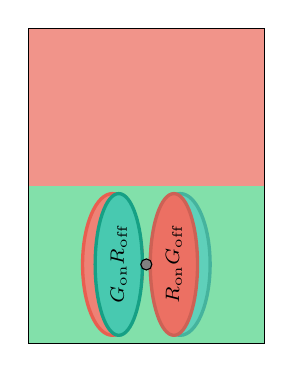
\begin{tikzpicture}
            \fill[alizarin!60]                                            (-1.50, 2.00) rectangle (1.50, 0.00);
            \fill[emerald!60]                                             (-1.50,-2.00) rectangle (1.50, 0.00);
            \filldraw[color=greensea!80,    fill=turquoise!70, very thick]( 0.43,-1.00) ellipse   (0.38 and 0.90);
            \filldraw[color=alizarin!90,    fill=alizarin!70,  very thick](-0.43,-1.00) ellipse   (0.38 and 0.90);
            \filldraw[color=pomegranate!80, fill=alizarin!80,  very thick]( 0.35,-1.00) ellipse   (0.30 and 0.90)
                 node[color=black, anchor=center, rotate=90] {$\scriptstyle R_{\text{on}}G_{\text{off}}$};
            \filldraw[color=greensea,       fill=turquoise!80, very thick](-0.35,-1.00) ellipse   (0.30 and 0.90)
                 node[color=black, anchor=center, rotate=90] {$\scriptstyle G_{\text{on}}R_{\text{off}}$};
            \filldraw[color=black,          fill=gray]                    ( 0.00,-1.00) circle    (2pt);
            \draw (current bounding box.north east) rectangle (current bounding box.south west);
            \end{tikzpicture}
        \caption{Minor Response}
    \end{subfigure}%
    \par \bigskip
    \begin{subfigure}{0.3\textwidth}
        \centering
        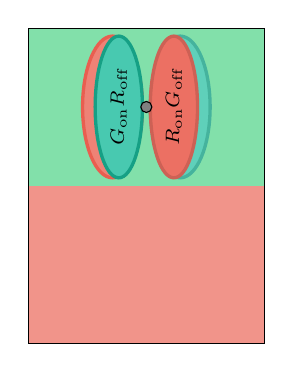
\begin{tikzpicture}
            \fill[emerald!60]                                             (-1.50, 2.00) rectangle (1.50, 0.00);
            \fill[alizarin!60]                                            (-1.50,-2.00) rectangle (1.50, 0.00);
            \filldraw[color=greensea!80,    fill=turquoise!70, very thick]( 0.43, 1.00) ellipse   (0.38 and 0.90);
            \filldraw[color=alizarin!90,    fill=alizarin!70,  very thick](-0.43, 1.00) ellipse   (0.38 and 0.90);
            \filldraw[color=pomegranate!80, fill=alizarin!80,  very thick]( 0.35, 1.00) ellipse   (0.30 and 0.90)
                 node[color=black, anchor=center, rotate=90] {$\scriptstyle R_{\text{on}}G_{\text{off}}$};
            \filldraw[color=greensea,       fill=turquoise!80, very thick](-0.35, 1.00) ellipse   (0.30 and 0.90)
                 node[color=black, anchor=center, rotate=90] {$\scriptstyle G_{\text{on}}R_{\text{off}}$};
            \filldraw[color=black,          fill=gray]                    ( 0.00, 1.00) circle    (2pt);
            \draw (current bounding box.north east) rectangle (current bounding box.south west);
        \end{tikzpicture}
        \caption{Minor Response}
    \end{subfigure}%
    \begin{subfigure}{0.3\textwidth}
        \centering
            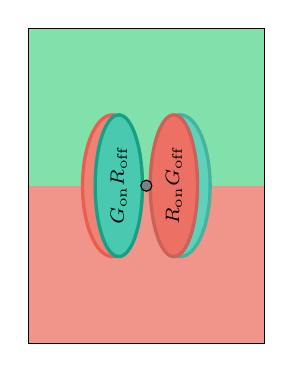
\begin{tikzpicture}
            \fill[emerald!60]                                             (-1.50, 2.00) rectangle (1.50, 0.00);
            \fill[alizarin!60]                                            (-1.50,-2.00) rectangle (1.50, 0.00);
            \filldraw[color=greensea!80,    fill=turquoise!70, very thick]( 0.43, 0.00) ellipse   (0.38 and 0.90);
            \filldraw[color=alizarin!90,    fill=alizarin!70,  very thick](-0.43, 0.00) ellipse   (0.38 and 0.90);
            \filldraw[color=pomegranate!80, fill=alizarin!80,  very thick]( 0.35, 0.00) ellipse   (0.30 and 0.90)
                 node[color=black, anchor=center, rotate=90] {$\scriptstyle R_{\text{on}}G_{\text{off}}$};
            \filldraw[color=greensea,       fill=turquoise!80, very thick](-0.35, 0.00) ellipse   (0.30 and 0.90)
                 node[color=black, anchor=center, rotate=90] {$\scriptstyle G_{\text{on}}R_{\text{off}}$};
            \filldraw[color=black,          fill=gray]                    ( 0.00, 0.00) circle    (2pt);
            \draw (current bounding box.north east) rectangle (current bounding box.south west);
            \end{tikzpicture}
        \caption{Minimal Response}
    \end{subfigure}%
    \begin{subfigure}{0.3\textwidth}
        \centering
            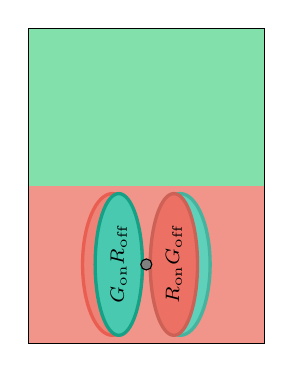
\begin{tikzpicture}
            \fill[emerald!60]                                             (-1.50, 2.00) rectangle (1.50, 0.00);
            \fill[alizarin!60]                                            (-1.50,-2.00) rectangle (1.50, 0.00);
            \filldraw[color=greensea!80,    fill=turquoise!70, very thick]( 0.43,-1.00) ellipse   (0.38 and 0.90);
            \filldraw[color=alizarin!90,    fill=alizarin!70,  very thick](-0.43,-1.00) ellipse   (0.38 and 0.90);
            \filldraw[color=pomegranate!80, fill=alizarin!80,  very thick]( 0.35,-1.00) ellipse   (0.30 and 0.90)
                 node[color=black, anchor=center, rotate=90] {$\scriptstyle R_{\text{on}}G_{\text{off}}$};
            \filldraw[color=greensea,       fill=turquoise!80, very thick](-0.35,-1.00) ellipse   (0.30 and 0.90)
                 node[color=black, anchor=center, rotate=90] {$\scriptstyle G_{\text{on}}R_{\text{off}}$};
            \filldraw[color=black,          fill=gray]                    ( 0.00,-1.00) circle    (2pt);
            \draw (current bounding box.north east) rectangle (current bounding box.south west);
            \end{tikzpicture}
        \caption{Minor Response}
    \end{subfigure}
    \caption{A double-opponent cell selective to vertically oriented borders with red to the right and green on the left; completely unresponsive to a horizontal border. While its $R_{\text{on}}$ receptive field might be strongly stimulated in (a) and (f), it's $R_{\text{off}}$ receptive field cancels it out. Similarly, in (c) and (d) its $G_{\text{on}}$ receptive field is stimulated but cancelled out by activity in its $G_{\text{off}}$ receptive field. In (b) and (e) both of its $R_{\text{on}}$ and $G_{\text{on}}$ receptive fields are moderately activated, but again, cancelled out by activation in its $R_{\text{off}}$ and $G_{\text{off}}$ receptive fields, respectively.}
\end{figure}

\end{document}